\documentclass{beamer}

\usepackage[english]{babel}
\usepackage[utf8]{inputenc}

\usetheme[%
  %nexus,%        Nexus Fonts benutzen
  %lnum,%         Versalziffern verwenden
  %cmyk,%<rgbprint>,          Auswahl des Farbmodells
  orange,%<orange/green/violet> Auswahl des Sekundärfarbklangs
  light,%<light,medium>        Auswahl der Helligkeit
  colorhead,%    Farbig hinterlegte Kopfleiste
  colorfoot,%    Farbig hinterlegt Fußleiste auf Titelseite
  colorblocks,%   Blöcke Farbig hinterlegen
  %nopagenum,%    Keine Seitennumer in Fußzeile
  %totalpages,%    Angabe der Gesamtseitenzahl in Fußzeile
  nodate,%       Kein Datum in Fußleiste
  %tocinheader,%   Inhaltsverzeichnis in Kopfleiste
  %tinytocinheader,% kleines Kopfleisten-Inhaltsverzeichnis
  %widetoc,%      breites Kopfleisten-Inhaltsverzeichnis
  %narrowtoc,%    schmales Kopfleisten-Inhaltsverzeichnis
  %nosubsectionsinheader,%  Keine subsections im Kopfleisten-Inhaltsverzeichnis
  nologoinfoot,% Kein Logo im Fußbereich darstellen
  ]{tubs}
\usepackage{tikz}
\usetikzlibrary{arrows.meta}

% BibLatex configuration
\usepackage{csquotes}
\usepackage[backend=biber,style=authoryear,giveninits=true,url=false,doi=false,isbn=false]{biblatex}
\addbibresource{bibliography.bib}
\setbeamertemplate{bibliography item}[text]

\setbeamertemplate{theorems}[numbered]
\setbeameroption{show notes}

% Titelseite
\title{Reducing fermion density matrices: a geometric view}
\subtitle{\hfill Joint work with V. Bach}
\author{R. Rauch}
\date{Singapore, September 13, 2019}
\titlegraphic[scaled]{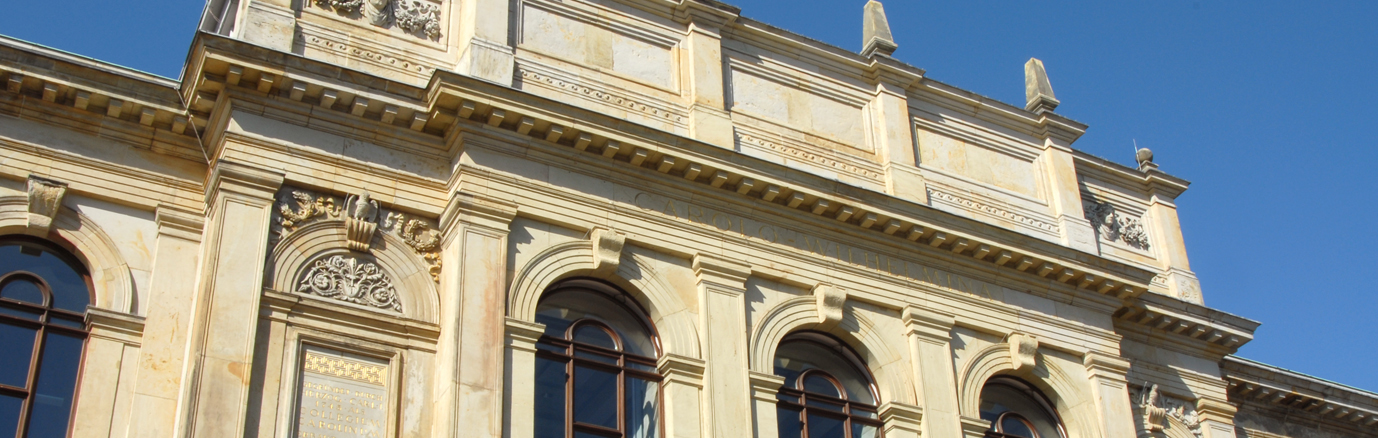
\includegraphics{titlepicture.jpg}}

\DeclareMathOperator{\tr}{tr}
\DeclareMathOperator{\pos}{pos}
\DeclareMathOperator{\spn}{span}
\DeclareMathOperator{\im}{im}
\newcommand{\IN}{\ensuremath{\mathbb{N}}}
\newcommand{\IZ}{\ensuremath{\mathbb{Z}}}
\newcommand{\IR}{\ensuremath{\mathbb{R}}}
\newcommand{\IC}{\ensuremath{\mathbb{C}}}
\newcommand{\IK}{\ensuremath{\mathbb{K}}}
\newcommand{\normord}[1]{:\mathrel{#1}:}
\newcommand{\card}[1]{{\ensuremath{\left|#1\right|}}}
\newcommand{\imag}{\mathrm{i}}
\newcommand{\CAR}[1]{{\ensuremath{\IC[c,c^*]}}}
\newcommand{\CARabs}[1]{{\ensuremath{\mathfrak{A}(#1)}}}
\newcommand{\one}{\mathbb{1}}
\newcommand{\N}{\mathbf{n}}
\newcommand{\C}{\mathbf{c}}
\newcommand{\Cd}{\C^*}
\newcommand{\PowerSet}[1]{\mathfrak{P}\left(#1\right)}
\newcommand{\HS}{{\mathcal{L}^2(\FockSpace)}}
\newcommand{\HSbasis}{\mathfrak{B}}
\newcommand{\HilbertSpace}{\ensuremath{\mathfrak{h}}}
\newcommand{\FockSpace}{\mathcal{F}}
\newcommand{\Vacuum}{\Omega_\FockSpace}
\newcommand{\sign}[2]{\begin{bmatrix}\begin{matrix}#1\end{matrix}\\\begin{matrix}#2\end{matrix}\end{bmatrix}}
\newcommand{\Hamiltonian}{\mathbb{H}}
\newcommand{\StateSpace}{\mathcal{S}}
\newcommand{\DensityMatrices}{\mathcal{D}}

% space of k-body operators
\newcommand{\kbOp}[1][k]{{\ensuremath{\mathcal{O}_{#1}}}}
\newcommand{\PkbOp}[1][k]{{\ensuremath{\pi_{#1}}}}
\newcommand{\kbOpBasis}[1][k]{\mathfrak{B}_{#1}}

% space of k-body observables
\newcommand{\kbOb}[1][k]{{\ensuremath{\mathcal{O}_{#1}^\mathbb{R}}}}
\newcommand{\PkbOb}[1][k]{{\ensuremath{\pi_{#1}^\mathbb{R}}}}
\newcommand{\kbObBasis}[1][k]{\mathfrak{B}_{#1}}

\begin{document}

\begin{frame}[plain]
\titlepage
\end{frame}

\begin{frame}{Overview}
  \begin{itemize}
    \item \textbf{Scope}: finite-dimensional, fermion many-particle systems
    \item \textbf{Outline}:
      \begin{enumerate}
        \item Give a geometric view on
          \begin{itemize}
            \item reduced density matrices,
            \item the representability problem and
            \item representability conditions.
          \end{itemize}
        \item Orthogonalization results \parencite{Bach2019}
      \end{enumerate}
  \end{itemize}
\end{frame}

\section{Motivation: The Representability Problem}
\subsection{Quantum Systems in Theoretical Chemistry}
\frame{\sectionpage}

\begin{frame}{Molecules in Quantum chemistry}
    \begin{itemize}
        \item<1-> \textbf{Hilbert space:} Fermion Fock space
        \begin{equation}
            \mathcal{F}=\bigoplus_{N\ge 0}\bigwedge^N\HilbertSpace\qquad
            \begin{gathered}
                \text{with }\HilbertSpace=\text{ $1$-particle Hilbert space},\\
                \text{e.g. }\HilbertSpace=L^2(\IR^3)\otimes\IC^2.
            \end{gathered}
        \end{equation}
        \item<2-> \textbf{States:} density matrices on $\FockSpace$, i.e.
        \begin{equation}
            \DensityMatrices=\{\rho\in\mathcal{B}(\FockSpace)\mid \rho\ge 0, \tr\{\rho\}=1\}.
        \end{equation}
        \item<3-> \textbf{Hamiltonian:} a \emph{2-body operator} $\Hamiltonian=\Hamiltonian^*=\bigoplus_{N\ge 0}\Hamiltonian_N$, e.g.
        \begin{equation}
            \Hamiltonian_N=
            \underbrace{\sum_{i=1}^N\left(-\Delta_i-\sum_{j=1}^K\frac{Z_j}{|x_i-R_j|}\right)}_{\text{1-particle free part}}
            +\underbrace{\sum_{1\le i<j\le N}\frac{1}{|x_i-x_j|}}_{\text{2-particle interaction part}}.
        \end{equation}
    \end{itemize}
\end{frame}

\subsection{Reducing States: The Representability Problem}
\begin{frame}{Computing the Ground State Energy}
    \begin{block}{}<1->
        \textbf{Key Problem}: Compute the ground state energy
        \begin{equation}
            \label{GSE}
            E_0=\inf_{\rho\in\DensityMatrices}\tr\{\rho\Hamiltonian\}
            \visible<5->{
              \alert{=\inf_{r\in\pi_2(\DensityMatrices)}\tr\{r\Hamiltonian\}.}
            }
        \end{equation}
    \end{block}
    \begin{itemize}
        \item<2-> \textbf{Observe}: For $2$-body Hamiltonians $\Hamiltonian$ the variation over
        $\DensityMatrices$ is very inefficient:
        \begin{itemize}
            \item<3-> General density matrix $\rho$ contains ``too much'' information,
            \item<3-> we only need expectation values of $2$-body operators.
        \end{itemize}
      \item<4-> \textbf{Idea}: Replace $\rho$ by its \emph{2-body-reduction} $\PkbOp[2](\rho)$.
    \end{itemize}
\end{frame}

\begin{frame}{Geometric definition of $\PkbOp[2](\rho)$}
    \begin{definition}[\cite{Erdahl1978}]
      Let $k\in\IN_0$ and $\kbOp$ the space of $k$-body operators on $\FockSpace$. Define
      \begin{equation}
        \PkbOp:\HS\to\HS
      \end{equation}
      as the orthogonal projection onto $\kbOp$.
    \end{definition}
    \begin{itemize}
      \item Orthogonality is understood with respect to the Hilbert-Schmidt
        scalar product $\langle a,b\rangle_{\HS}=\tr\{a^*b\}$.
      \item This definition only makes sense if $\dim\HilbertSpace<\infty$!
      \item This definition ensures that
        \begin{equation}
          \tr\{\rho\Hamiltonian\}=\tr\{\PkbOp(\rho)\Hamiltonian\}
          \qquad\forall\Hamiltonian\in\kbOp.
        \end{equation}
    \end{itemize}
\end{frame}

\begin{frame}{The Representability Problem}
    \begin{block}{Representability Problem (for $\PkbOp[2](\DensityMatrices)$)}
        Find a \emph{computationally efficient} characterization of
        $\PkbOp[2](\DensityMatrices)$.
    \end{block}
    \onslide<2->{
        \begin{center}
        \begin{tikzpicture}[scale=.6]
            % Convex set of density matrices
            -- (-1,4) -- (-1.75,2) -- cycle;
            \filldraw[fill=tubsGray!20, very thick, rotate=30] (1, 2) ellipse (3.2 and 2.2);
            \draw (.2,2.2) node {$\DensityMatrices$};

            % Subspace of $k$-body operators
            \draw (8,-.74) node[below] {$\kbOp[2]$} -- (8,5.2);

            % Set or representable density matrices
            \draw[very thick,color=tubsRed] (8,-.28) -- node[left=5pt]{$\PkbOp[2](\DensityMatrices)$} (8,4.74);

            \draw[dashed] (.7,4.74) -- (8,4.74);
            \draw[dashed] (-1,-.28) -- (8,-.28);
        \end{tikzpicture}
        \end{center}
    }
\end{frame}
\begin{frame}{The dual problem: representability conditions}
  \begin{theorem}[\cite{Garrod1964, Kummer1967}]
    For $r\in\kbOp[2]$ with $\tr(r)=1$ the following conditions are equivalent:
    \begin{enumerate}
      \item $r\in \PkbOp[2](\DensityMatrices)$, i.e. $r$ is \emph{representable},
      \item for all $\xi\in\kbOp[2]$ with $\xi\ge 0$ we have $\langle r,\xi\rangle_\HS\ge 0$.
    \end{enumerate}
  \end{theorem}
  \begin{itemize}
    \item Elements of $\mathcal{R}_2:=\left\{\xi\in\kbOp[2]\mid\xi\ge 0
      \right\}$ are called \emph{representability conditions}.
    \item They provide \emph{necessary} conditions for representability.
    \item Characterizing $\mathcal{R}_2$ is called the \emph{dual} representability problem.
  \end{itemize}
\end{frame}

\begin{frame}{Geometric interpretation}
  \begin{itemize}
    \item Representability conditions = \emph{supporting hyperplanes} of $\PkbOp[2](\DensityMatrices)$.
  \end{itemize}
  \begin{center}
  \begin{tikzpicture}[scale=.6]
      % Convex set of reduced density matrices
      \filldraw[fill=tubsGray!20,very thick] (0,0) -- (2,0.5) -- (3,2.5) .. controls (2.8,4.5) .. (1,5)
      -- (-1,4) -- (-1.75,2) -- cycle;
      \draw (.8,2.5) node {$\PkbOp[2](\DensityMatrices)$};

      % Some representability conditions
      \draw[very thick,color=tubsRed] (1.5,-1) node[below] {$\xi_1^\perp$} -- (4.2,3.8);
      \draw[very thick,color=tubsRed] (4.5,1.5) node[below] {$\xi_2^\perp$} -- (1.8,6);
      \draw[very thick,color=tubsRed] (-2,5.2) node[left] {$\xi_3^\perp$} -- (3.2, 5.2);
  \end{tikzpicture}
  \end{center}
\end{frame}

\begin{frame}{Lower bound methods}
  \begin{corollary}[Lower-bound methods]
    Let $\mathcal{X}\subseteq\mathcal{R}_2$ be a set of representability conditions and
    $\Hamiltonian\in\kbOp[2]$. Then
    \begin{equation}
      E_0(\Hamiltonian)\ge\inf_{\substack{r\in\kbOp[2],\tr(r)=1\\\langle r,\mathcal{X}\rangle \ge 0}}\tr\{r\Hamiltonian\}
      \label{1fe38fbd}
    \end{equation}
  \end{corollary}
  \begin{itemize}
    \item \textbf{Open Question}: Given a particular $\Hamiltonian\in\kbOp[2]$,
      how find $\mathcal{X}\subseteq\mathcal{R}_2$ s.t.
      \begin{enumerate}
        \item the variation \eqref{1fe38fbd} can be computed efficiently and
        \item the error in \eqref{1fe38fbd} is small?
      \end{enumerate}
  \end{itemize}
\end{frame}

\begin{frame}{Some History of Representability Methods}
    \begin{itemize}
        \item \textbf{1940:} Idea to replace $\DensityMatrices$ by $R_2(\DensityMatrices$) (Husimi)
        \item \textbf{1950/60s:} First systematic analysis (Coleman, Coulson, Garrod, Percus, Löwdin, Yang)
        \begin{itemize}
            \item $GPQ$-conditions lead to inaccurate lower bounds
            \item solved Representability Problem for $R_1(\mathcal{SD}_N)$
        \end{itemize}
        \item \textbf{1978:} $T_1$- and $T_2$-conditions (Erdahl)
        \item \textbf{2005:} Representability of $R_1(\mathcal{P}_N)$ solved  (Klyachko)
        \item \textbf{2006:} Highly accurate lower bounds exploiting Erdahls $T_1$- and $T_2$-conditions (Cancés, Lewin, Stoltz)
        \item \textbf{2012:} Derivation of HF error estimates from $G$- and $P$-condition (Bach, Bretaux, Knörr, Menge)
    \end{itemize}
\end{frame}

\section{Orthogonalization of $k$-body operators}\frame{\sectionpage\fullcite{Bach2019}}
\subsection{Goal}
\begin{frame}{Overview}
\begin{itemize}
    \item \textbf{Goal}: Find a more explicit formula for $\pi_k$
    \item<3-> \textbf{Approach:} construct an explicit orthonormal basis of $\kbOp$.
    \begin{enumerate}
        \item Choose some (non-orthonormal) basis of $\kbOp$.
        \item Apply Gram-Schmidt orthogonalization in low-dimensional examples.
        \item Find and prove a general conjecture.
    \end{enumerate}
\end{itemize}
\end{frame}

\subsection{Results}
\begin{frame}{Main Result}
    \begin{theorem}[\cite{Bach2019}]
        Let $\dim\HilbertSpace\doteq n<\infty$ and $\varphi_1,\ldots,\varphi_n$ an ONB of $\HilbertSpace$.
        Then an orthogonal basis of $\HS$ is given by
        \begin{equation}
            \HSbasis\doteq\left\{
              \left.\sum_{L\subseteq K}(-2)^Lc_I^*c_L^*c_Lc_J\;\right|
            \begin{gathered}
                I,J,K\subseteq\{1,\ldots,n\}\\\text{ mutually disjoint}
            \end{gathered}
            \right\},
        \end{equation}
        where for $I=\{i_1<\cdots<i_l\}\subseteq\{1,\ldots,n\}$ we define
        \begin{align}
            c_I^*&\doteq c^*(\varphi_{i_1})\cdots c^*(\varphi_{i_l}),&
            c_I&\doteq\left(c_I^*\right)^*=c(\varphi_{i_l})\cdots c(\varphi_{i_1}).
        \end{align}
    \end{theorem}
\end{frame}

\begin{frame}{Main Result: Geometric Interpretation}
    \begin{corollary}[\cite{Bach2019}]
        An orthogonal basis of $\kbOp$ is given by $\HSbasis\cap\kbOp$.
    \end{corollary}
    \begin{figure}
    \begin{tikzpicture}[scale=.6]
        % Convex set of density matrices
        -- (-1,4) -- (-1.75,2) -- cycle;
        \filldraw[fill=tubsGray!20, very thick, rotate=30] (1, 2) ellipse (3.2 and 2.2);
        \draw (.2,2.2) node {$\DensityMatrices$};

        % Subspace of $k$-body operators
        \draw (8,-.74) node[below] {$\kbOp[2]$} -- (8,5.2);

        \draw[dashed] (.7,4.74) -- (8,4.74);
        \draw[dashed] (-1,-.28) -- (8,-.28);

        % visualize basis
        \draw[Stealth-Stealth, color=tubsRed, very thick] (8,1.72) -- node[left, near end]{$\HSbasis$} (8,-.28) -- (6,-.28);
    \end{tikzpicture}
\end{figure}
\end{frame}

\begin{frame}{Application: Expansion of $\pi_k$}
  \begin{corollary}
    Let $a\in L(\FockSpace)$ be particle-number preserving, i.e. $[a,\hat{\IN}]=0$. Then
    \begin{equation}
      2^n\pi_1(a)=4d\Gamma(\gamma_a)-2\tr(a)\hat{\IN}-2\tr(\gamma_a)+(n+1)\tr(a).
    \end{equation}
  \end{corollary}
  \textbf{Notation}:
  \begin{itemize}
    \item $\gamma_a\in L(\HilbertSpace)$ denotes the usual 1-RDM of $a$
    \item $d\Gamma$ denotes the (differential) second quantization, e.g. $\hat{\IN}=d\Gamma(1_\HilbertSpace)$
  \end{itemize}
\end{frame}

\begin{frame}{Ongoing Work}
  \begin{itemize}
    \item \textbf{Observe}: Representability conditions $\mathcal{R}_k$ invariant under \emph{Bogoliubov transformations}
    \item \textbf{Question}: Can we classify rep. conditions modulo Bog. transformations, i.e.
      \begin{equation*}
        \mathcal{R}_k/\operatorname{Bog}(\FockSpace)=\;?
      \end{equation*}
  \end{itemize}
\end{frame}

\begin{frame}
  \begin{center}
    {\Huge Thank You!}
  \end{center}
\end{frame}

\section{Appendix}
\frame{\sectionpage}

\begin{frame}{$k$-Body Operators}
\begin{definition}
    A \emph{$k$-body operator} on $\FockSpace$ is a $\IC$-linear
    combination of elements of the form
    \begin{equation}
        c^\sharp(f_1)\cdots c^\sharp(f_{2l})\qquad f_1,\ldots,f_{2\ell}\in\HilbertSpace
        \text{ and }0\le \ell\le k,
    \end{equation}
    with $c^*(f),c(f)\in\mathcal{B}(\FockSpace)$ the \emph{creation-} and
    \emph{annihilation operators} on $\FockSpace$.
\end{definition}
\end{frame}

\begin{frame}{Representability of $R_2(\DensityMatrices_N)$}
    \begin{exampleblock}{}
        Let $\rho\in\DensityMatrices_N\doteq\{\rho\in\DensityMatrices\mid\hat{\IN}\rho=N\rho\}$. Then $R_2(\rho)\in\kbOp[2]'$
        is characterized by
        \begin{align}
            \gamma_\rho&\in\mathcal{B}(\HilbertSpace),\tag{1-RDM}\\
            \Gamma_\rho&\in\mathcal{B}(\HilbertSpace\wedge\HilbertSpace).\tag{2-RDM}
        \end{align}
    \end{exampleblock}
    \begin{itemize}
        \item \textbf{$N$-Representability Problem}: Given $\gamma\in\mathcal{B}(\HilbertSpace)$
        and $\Gamma\in\mathcal{B}(\HilbertSpace\wedge\HilbertSpace)$,  is there $\rho\in\DensityMatrices$ with $\hat{\IN}\rho=N\rho$ such that
            \begin{align}
                \gamma&=\gamma_\rho&\Gamma&=\Gamma_\rho
            \end{align}
        \item Examples of \textbf{$N$-Representability conditions}:
        \begin{equation}
            \begin{aligned}
                0&\le\gamma_\rho\le 1,&
                \tr\{\gamma_\rho\}&=N,&
                \Gamma_\rho&\ge 0.
            \end{aligned}
        \end{equation}
    \end{itemize}
\end{frame}

\subsection{Current Research}
\begin{frame}{Current Research}
    \begin{enumerate}
        \item Characterize $\pi_k(\DensityMatrices)\subseteq\kbOp$ using the ONB $\HSbasis\cap\kbOp$
        \item Identify classical representability conditions as boundary conditions
        \item Obtain new representability conditions
        \item Study action of Bogoliubov transformations on representability conditions
    \end{enumerate}
\end{frame}

\begin{frame}{Possible Application}
    \begin{itemize}
        \item Consider a 2-body Hamiltonian $\Hamiltonian$, fix an ONB
        $\varphi_1,\dots,\varphi_n$ of $\HilbertSpace$ and write
        \begin{equation}
            \Hamiltonian=\sum_{i,j}t_{ij}c_i^*c_j+\frac{1}{2}\sum_{i,j,k,l}V_{ij;kl}c_i^*c_j^*c_lc_k,
        \end{equation}
        \item Let $\mathfrak{B}$ be the associated ONB of $\HS$ as given by Theorem 1
        \item For $\mathfrak{A}\subseteq\mathfrak{B}$ define
        $P_{\mathfrak{A}}\doteq\sum_{\theta\in\mathfrak{A}}\left|\theta\rangle\langle\theta\right|\le
        1_\HS$.
        \item Then, under suitable positivity requirements on $V$,
        \begin{equation}
            \Hamiltonian\ge\sum_{i,j}t_{ij}c_i^*c_j+
            \frac{1}{2}\sum_{i,j,k,l}V_{ij;kl}c_i^*c_j^*\textcolor{red}{P_\mathfrak{A}}c_lc_k
            \doteq\Hamiltonian_\mathfrak{A}.
        \end{equation}
        \item \textbf{Idea:} by a suitable choice
        of the orbital basis $\varphi_1,\ldots,\varphi_n$ and $\mathfrak{A}\subseteq\mathfrak{B}$
        one obtains nontrivial lower bound $E_0(\Hamiltonian_\mathfrak{A})$ of $E_0(\Hamiltonian)$.
    \end{itemize}
\end{frame}

\section*{References}
\begin{frame}[allowframebreaks]{References}
    \nocite{*}
    \printbibliography
\end{frame}

\end{document}
